\cotefile{29}
\scanpage{95}
% Image orientation: the typescript is upside down in the supplied scan.
% archive foliation: 94
tera donc du a) dans le

\uline{Corollaire} 3.2. Soit\inserted{\unsure{en}} $S$ un préschéma non vide, $u:M'\quad M$ un homomorphisme de groupes commutatifs ordinaires, $u':G\quad G'$ l'homomorphisme transposé. Alors :
% Blank connector positions in this carbon typescript are retained as spaces.

a) Pour que $u$ soit un monomorphisme, il f et s que $u'$ soit fidèlement plat.

b) Pour que $u$ soit un épimorphisme, il f et s que $u'$ soit un monomorphisme (et alors $u'$ est même une immersion fermée).

Pour prouver a), on note que si $u$ est un monomorphisme, alors $\underline{O}_S(M)$ est un Module \deleted{\unsure{libre sur}}\inserted{sur} $\underline{O}_S(M')$, \deleted{\unsure{tout système de représentants}} admettant une base non vide (savoir, le système de sections défini par n'importe quel système de représentants dans $M$ modulo $M'$), à fortiori il est fidèlement plat. Réciproquement, s'il en est ainsi, alors $\underline{O}_S(M')\quad\underline{O}_S(M)$ est injectif, ce qui (pour $S\ne\varnothing$) implique que $u:M'\quad M$ est injectif.

Pour prouver b), on note que si $u$ est un épimorphisme, alors $\underline{O}_S(M')\quad\underline{O}_S(M)$ est surjectif, donc $u'$ est une immersion fermée et à fortiori un monomorphisme. Inversement, s'il en est ainsi, alors $\operatorname{Ker}u'={}$ groupe unité, or \deleted{\unsure{posant}} posant $M''=\operatorname{Coker}u$, on a vu que $\operatorname{Ker}u'\quad D_S(M'')$, donc par 2.1. d) on a $M''=0$ donc $u$ est un épimorphisme.

On conclut de 3.1. de la façon habituelle:

\uline{Corollaire} 3.3. Soit
\diagram{\begin{tikzcd}[column sep=small]
M' \arrow[r,phantom,"u"] & M \arrow[r,phantom,"v"] & M''
\end{tikzcd}}
une suite exacte de groupes commutatifs ordinaires, considérons la suite transposée
\diagram{\begin{tikzcd}[column sep=small]
G'' \arrow[r,phantom,"v'"] & G \arrow[r,phantom,"u'"] & G'.
\end{tikzcd}}
Alors $v'$ induit un morphisme fidèlement plat et quasi-compact de $G''$ dans $\operatorname{Ker}u'$, et ce dernier est un groupe diagonalisable.
\scanpage{96}
\mspage{5}
% archive foliation: 95
\margin{on ait $n\gamma=\sum_0^{\unsure{r}}c_i\beta_i$}

On utilise maintenant \unsure{la théorie|le théorie} de Kummer pour $\mathcal{X}/D$ pour trouver un \unsure{revêtement|extension} de $\mathcal{X}/D_0$ qui ait comme groupe \uline{\unsure{d'inertie}} \unsure{de Galois} $J_0\inserted{\simeq\unsure{\mu_t^\infty}}$ \unsure{égal au} groupe d'inertie en $X_0$ .....

\margin{$\unsure{\beta^0}=n\gamma+\sum_1^r c_i\unsure{\beta^i}$\par $\unsure{\partial\simeq K^{\mathrm{ab}}}$}

\diagram{\begin{tikzcd}[column sep=small]
\unsure{\Pi|\pi}_2^t(X_0/D'_0,\bar\xi_0) \arrow[r] \arrow[r,shift right=4ex,draw,{Bar}-{Bar},start anchor=south,end anchor=south] &
\mu_{X_0,t}^{\infty}(\bar\xi_0) \arrow[r] &
\unsure{\Pi|\pi}_1^t(\mathcal{X}/D,\bar\xi_1) \arrow[r] &
\unsure{\Pi|\pi}_1^t(X_0/D'_0,\bar\xi_0) \arrow[r] \arrow[ll,bend right=60,start anchor=north,end anchor=north] & 0
\end{tikzcd}}

$\unsure{\Pi|\pi}_1^t(\mathcal{X}/D,\bar\xi_1)$ comme extension de $\unsure{\Pi|\pi}_1^t(X_0/D'_0,\bar\xi_0)$ est connu \unsure{entièrement} en termes de $X_0/D'_0$ et de la classe $\alpha\in H^2(X_0\deleted{-\unsure{D_0}},\mu_{X_0,\mathrm{tame}}^\infty)$ [self-intersection de $X_0$ dans $\mathcal{X}$] ....

\uline{Exemple I} $X_0$ courbe algébrique\inserted{lisse} sur $k$ alg. clos.

Alors $\unsure{\Pi|\pi}_2^t(X_0-D'_0)=0$ sauf si $X_0\simeq\mathbf{P}^1_k$\inserted{, $D'_0=\varnothing$}, en quel cas $\unsure{\Pi|\pi}_2^t(X_0,\bar\xi_0)\simeq\mu_{X_0,t}^{\infty}(\bar\xi_0)$. L'hom $\mathbf{Z}\longrightarrow\mu_t^{\deleted{\unsure{2}}\infty}$ dans ce dernier cas correspond \unsure{exactement} à la \uline{multiplication} par $\unsure{n}$ (le degré). \deleted{\unsure{En tout cas}}

1°) \inserted{$\boxed{X_0-D'_0\ne\mathbf{P}^1_k}$}\deleted{\illegible{2}} $\unsure{\Pi|\pi}_1^t(\mathcal{X}/D,\bar\xi_{\unsure{1}})$ est une extension \uline{triviale} de $\unsure{\Pi|\pi}_1^t(X_0-D_0,\bar\xi_0)$ par $\mu_t^\infty(\bar\xi_0)$.
\scanpage{97}
% Image orientation: upside-down typescript; archive foliation: 96.
\uline{Corollaire} 3.4. Soient $S$ un préschéma, $u:G\quad H$ un homomorphisme de \deleted{\unsure{$S$-groupes}} $S$-préschémas en groupes localement diagonalisables,\inserted{avec $H$ de type fini sur $S$} Alors:

a) $G'=\operatorname{Ker}u$ est localement diagonalisable, il est de type fini sur $S$ si $G$ l'est.

b) Le quotient $G/G'$ existe, de façon plus précise la relation d'équivalence définie par $G'$ dans $G$ est effective pour la descente fidèlement plate quasi-compacte (cf exposé IV). De plus $\unsure{G/G'}$ est localement diagonalisable.

c) \deleted{Par \unsure{suite} (\unsure{image})} L'homomorphisme $u:G\quad H$ se factorise de façon unique en
\diagram{\begin{tikzcd}[column sep=small]
G \arrow[r,phantom,"v"] & G/G' \arrow[r,phantom,"w"] & H
\end{tikzcd}}
, où $v$ est l'homomorphisme canonique (donc $v$ est fidèlement plat et quasi-compact)\deleted{\unsure{et}} De plus $w$ est une immersion fermée, et à fortiori un monomorphisme.

La première assertion de c) est conséquence de b), par définition du quotient $G/G'$. Comme toutes les assertions faites sont de nature locale sur $S$, on peut alors supposer $G$ et $H$ \deleted{\unsure{définis par}} diagonalisables, \deleted{\unsure{définis}} de la forme $D_S(M)$ et $D_S(N)$, et (compte tenu de 1.5.\inserted{qui implique $N$ de type fini} et 2.1. b)) $u$ défini par un homomorphisme $u':N\quad M$. Alors en vertu de 3.1. $G'$ est isomorphe à $D_S(\operatorname{Coker}u')$, ce qui prouve a). Pour prouver b) et c), il suffit de réaliser $G/G'$ comme $D_S(\operatorname{Im}u')$, en appliquant 3.3.

\uline{Remarques} Le résultat d'existence de quotients 3.4. sera substantiellement généralisé au N° suivant, \deleted{\unsure{ainsi que}} On notera que dans le présent N° et le précédent, l'hypothèse $S\ne\varnothing$ n'est intervenue que pour assurer la validité de certaines réciproques, \deleted{\unsure{affirmant que si $G=D_S$}} permettant de certaines hypothèses sur des schémas en groupes sur $S$, de conclure des propriétés correspondantes pour certains groupes ordinaires Les résultats en sens inverse sont valables sans restriction sur $S$, et les démonstrations données ici s'appliquent dans le cas général.
\scanpage{98}
\mspage{6}
% archive foliation: 97
2°) $\boxed{X_0-D'_0=\mathbf{P}^1_k}$ i.e. $X_0=\mathbf{P}^1_k$, $D'_0=\varnothing$. Alors \deleted{$\unsure{\Pi|\pi}_1^t(\unsure{X}/D,\bar\xi_1)$}\inserted{$\unsure{\Pi|\pi}_1^t(\underline{\mathcal{X}}/D,\bar\xi_1)$} est \deleted{une extension} isomorphe à $\mu_n(k)$, où $n$ est la partie première à $p=\operatorname{car}k$ du degré de la self-intersection $X_0.X_0$ dans $\mathcal{X}$.

\uline{Exemple} II a) $X_0=\operatorname{Spec}\mathbf{Z}$. Alors $\mu_{t,X_0}^\infty=0$,
\margin{\figure{\begin{tikzpicture}
\node[draw,ellipse,align=left,text width=7cm,inner sep=7pt] (n) at (0,0) {[\unsure{puisque} dans $X_0$ \unsure{tous|toutes} les car. résiduelles existent]};
\draw (n.south west) .. controls (-2,-0.8) and (-2.4,-1) .. (-2.2,-1.4);
\end{tikzpicture}}}
d'où
\[
\unsure{\Pi|\pi}_1^t(\mathcal{X}/D,\bar\xi_1)\simeq\unsure{\Pi|\pi}_1^t(X_0/D'_0,\bar\xi_0).
\]
\deleted{\unsure{Le pb de}} Si $D'_0=\varnothing$, on trouve $0$.

Si $D'_0\ne\varnothing$, la partie abélienne de $\unsure{\Pi|\pi}_1^t(X_0/D'_0,\bar\xi_0)$ est calculable par le corps des classes\inserted{$\bigl(\simeq\prod_{\ell\in D'_0}(\mathbf{Z}/\ell\mathbf{Z})^*\bigr)$}; \unsure{sans} doute $\unsure{\Pi|\pi}_1^t(X_0/D'_0,\bar\xi_0)$ \unsure{n'est} \unsure{en général pas} abélien fini. il y a des \deleted{\unsure{vraiment}} corps de nombres tamely ramifiés sur $\mathbf{Q}$, qui ne sont pas abéliens .... ??].
\margin{?}

b) $X_0=\operatorname{Spec}\mathbf{Z}-S$, $S\ne\varnothing$. Alors
\[
\mu_{t,X_0}^\infty=\prod_{\ell\in S}\mu^\infty(\ell)_{X_0}.
\]
Mais qu'est $\unsure{\Pi|\pi}_2^t(X_0/D'_0)$

???
\scanpage{99}
% Image orientation: upside-down typescript; archive foliation: 98.
\uline{Corollaire} 3.5. Soit $G$ un \deleted{\unsure{sché}} préschéma en groupes diagonalisable sur $S$, et soit $n$ un entier $\ne0$. Alors le sous-groupe ${}_n\unsure{H|G}$ de $G$ noyau de l'homomorphisme $n.\operatorname{id}_G:G\quad G$ est entier sur $S$, et fini sur $S$ si $G$ est de type fini sur $S$.

En effet, si $G=D_S(M)$; alors ${}_{\unsure{n}}G=D_S(M/nM)$ en vertu de 3.1., et on conclut par 2.1. c) c').

4. \uline{Fibrés principaux homogènes sous un groupe diagonalisable}.

Soient $S$ un préschéma, et $G=D_S(M)$ un groupe diagonalisable sur $S$. Nous nous proposons de déterminer les \uline{fibrés principaux homogènes} sur $S$, au sens de la ``topologie fidèlement plate quasi-compacte'', cf exposé IV. Comme $G$ lui-même est fidèlement plat et quasi-compact sur $S$, on sait par loc cit que ce sont exactement les $S$-préschémas\inserted{$P$}, \deleted{admettant}\inserted{formellement principaux} avec groupe d'opérateurs $G$, qui sont fidèlement plats et quasi-compacts sur $S$. Par définition, un $S$-préschéma Rappelons qu'un préschéma $P$ sur $S$, à groupes d'opérateurs $G$, est dit principal homogène si tout point de $S$ admet un voisinage ouvert $U$ et un morphisme fidèlement plat et quasi-compact $S'\quad U$, tel que $P'=P\times_S S'$ soit un fibré à opérateurs isomorphe à $G'=G\times_S S'$ (opérant sur lui-même par translations à droite). Comme $G$ est affine sur $S$, il en résulte par SGA VIII 5.6. que $P$ est nécessairement affine sur $S$. Notons aussi que puisque $G$ est lui-même fidèlement plat et quasi-compact sur $S$, $P$ est principal homogène sous $G$ sss il est ``formellement principal homogène'', et s'il est de plus fidèlement plat et quasi-compact sur $S$ (cf exposé IV).

Rappelons d'autre part (exposé I) que la donnée d'un $S$-préschéma $P$ \uline{affine sur} $S$ à groupe d'opérateurs $G=D_S(M)$ revient à la donnée d'une Algèbre quasi-cohérente \uline{graduée de type} $M$ sur $S$, i.e.
\scanpage{100}
% archive foliation: 99
\deleted{Il y a un s-groupe d'indice fini\inserted{$I'$} de \deleted{$\unsure{\Pi|\pi}_1(U)$}\inserted{$I$} qui opère sur $E$ via un pro-$\ell$-groupe. À fortiori,}
\deleted{\diagram{\begin{tikzcd}
I_0(\deleted{\unsure{\bar\xi}}) \arrow[r] \arrow[d] & I'_0 \arrow[d] \\
I(\deleted{\unsure{\bar\xi}}) \arrow[r] & I'
\end{tikzcd}}}

\figure{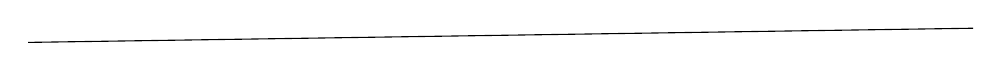
\begin{tikzpicture}[x=1cm,y=1cm]
\draw (0,0)--(12,.18);
\end{tikzpicture}}

\textcircled{a} Un résultat\inserted{local} de Abhyankar $\oplus$

\textcircled{b} \uline{Version \inserted{semi}globale du \deleted{\unsure{un}} résultat de Abhyankar}.

$X$ schéma loc. \unsure{n.th.} connexe

$\unsure{D}=\sum\unsure{D_i}$ diviseur\inserted{strictement} à croisements normaux

(composantes $Y_i$ \uline{régulières})

On suppose $Z=\bigcap_i\unsure{D_i}\ne\varnothing$, et que \deleted{\unsure{pour tt}}\inserted{le couple $(X,Z)$ est ``hensélien'', i.e. \unsure{pour} $\forall X'$ fini\inserted{sur $X$, conn $\ne\varnothing$}, \deleted{\unsure{l'image inverse} de $Z$ dans $X'$, $\unsure{\Pi|\pi}_0(\unsure{Z'})\simeq\unsure{\Pi|\pi}_0(X')$} $Z'$ est connexe $\ne\varnothing$}

\margin{\figure{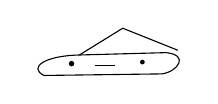
\begin{tikzpicture}[x=1cm,y=1cm]
\draw (0,.05) .. controls (-.2,.15) and (0,.3) .. (.45,.31) -- (1.55,.34) .. controls (1.85,.31) and (1.7,.1) .. (1.5,.07) -- cycle;
\fill (.35,.2) circle (.035); \fill (1.25,.22) circle (.03);
\draw (.65,.18)--(.9,.18);
\draw (.45,.31)--(1,.65)--(1.7,.37);
\end{tikzpicture}}}

\deleted{Alors} Soit \deleted{$\unsure{X}$} $U=X-\deleted{\unsure{supp}}Y$, $\xi$ un pt géom de $U$.

Alors a) $U$ connexe, et $\unsure{\Pi|\pi}_1(U,\xi)_t\longrightarrow\unsure{\Pi|\pi}_1(X,\xi)$ surjectif.

b) Pour tout $\unsure{D_i}$, le groupe d'inertie dans $\unsure{\Pi|\pi}_1(U,\xi)_t$ relatif \unsure{:|à} $\unsure{\Pi|\pi}_1(U)$ est un sous-groupe distingué \deleted{de $\unsure{\Pi|\pi}_1(U)\unsure{,\xi}$} commutatif $I_i$ de $Y_i$, \deleted{\unsure{on a}} et on a un épimorphisme canonique
\[
\deleted{\unsure{\xi}}
\prod_{\substack{\ell\ \text{inversible}\\\text{sur }\deleted{Z}\unsure{D_i}\\(\text{ou encore sur }Z)}}T_\ell(\Omega^*)\longrightarrow I_i.
\]

c) Les groupes $I_i$ commutent, et le \deleted{produit}\inserted{groupe engendré} est le noyau\inserted{$I$} de $\unsure{\Pi|\pi}_1(U,\xi)_t\unsure{-|\longrightarrow}\unsure{\Pi|\pi}_1(X,\xi)$.

a) Est immédiat.

b) L'image inverse de $\unsure{D_i}$ dans un rec. \deleted{\unsure{fini}}\inserted{connexe} \unsure{normal} modérément ramifié $X'$ de $X$ est normale (étude locale) et \uline{connexe}, \deleted{donc $I_i$ est} \unsure{irred}, donc $I_i$ est invariant. On sait bien qu'il est $\simeq$ quotient de $\prod_\ell T_\ell(\Omega^*)$, $\ell\ne\text{car. gén.}\text{ de }\unsure{D_i}$. Il faut prouver que $I$ est premier aux car. résiduelles en $\unsure{D_i}$. C'est une histoire locale sur $\unsure{D_i}$.

c) Commutation des $I_i$: \deleted{\unsure{Et.}} Étude locale en un pt de
\scanpage{101}
% archive foliation: 100
\textcircled{1}

$X$ schéma

$D_i$ diviseurs de Cartier $\geq0$ \hfill $1\leq i\leq r$

$n_i$ entiers $\geq1$ \hfill $1\leq i\leq r$

$\Gamma$ schém. en groupes sur $S$

$\deleted{\unsure{\mu=}}\mu_{\underline n}=\prod\mu_{n_i}$ \quad $(\underline n=(n_1,\ldots,n_r))$ sur $X$

Extension de groupes sur $X$
\diagram{\begin{tikzcd}[column sep=small]
1 \arrow[r] & \mu \arrow[r,dash] & G \arrow[r,dash] & \Gamma \arrow[r,dash] & 1
\end{tikzcd}}

\diagram{\begin{tikzcd}[column sep=small]
X' \arrow[r] & \widetilde X_{\unsure{1}} \arrow[r] & X
\end{tikzcd}}
morphisme de schémas sur $X$, à op. $G$.

On suppose a) que $G$ opère sur $\widetilde X_{\unsure{1}}$ que $\mu$ y opère trivialement, que \deleted{$\unsure{G}$} $\widetilde X_1$ devient \uline{torseur} sous $\Gamma$

b) En tant que fibré à opérateurs $\mu_{\widetilde X_{\unsure{1}}}\inserted{=\mu_{\underline n,\widetilde X}}$, $X'\unsure{/}$ sur $X$, est loc. \deleted{\unsure{à}} (sur $\widetilde X_{\unsure{1}}$) de type Kummérien relatif aux images inverses $\widetilde D_i$ des $D_i$ (supposés être encore diviseurs)\inserted{d'exposant $n_i$} i.e. de la forme
\[
\widetilde X[T_1,\ldots,T_r]/(T_1^{n_1}-a_1,\ldots,T_r^{n_r}-a_r),
\]
où les $a_i$ sont des équations des $\widetilde D_i$ (locales).

b$^2$) \deleted{$\Gamma$ opère sur $\mu$, \unsure{défini par}} On a donc un isom $\widetilde X\mathbin{\times}^{\Gamma}\mu\simeq\mu_n$.

\margin{\diagram{\begin{tikzcd}[column sep=small,row sep=small]
B_G \arrow[d] & B_\mu \arrow[l] \arrow[d] & B_{\unsure{\Gamma}}/(\widetilde X,\unsure{G}) \arrow[dl] \\
B_\Gamma & (\widetilde X,\Gamma) \arrow[l] \arrow[r,phantom,"\simeq"] & X
\end{tikzcd}}}

L'extension\inserted{$G$} de $\Gamma$ par $\mu$ définit une classe $\alpha\in H^2(B_\Gamma,\mu)\deleted{\unsure{\simeq\prod H^2(B_\Gamma,\mu_{n_i})}}$. On a un hom canonique, qui au\inserted{$\Gamma$-torseur} $X$
\diagram{\begin{tikzcd}[column sep=small,row sep=small]
H^2(B_\Gamma,\mu) \arrow[r,"\varphi"] & H^2(X,\mu_n) \arrow[r,phantom,"\simeq"] \arrow[d,phantom,"\unsure{\wr}"] & \prod H^2(X,\mu_{n_i}) \\
& H^2(B_\Gamma/(\widetilde X,\unsure{\Gamma}),\mu) &
\end{tikzcd}}

On veut prouver que \unsure{si}
\[
\varphi(\alpha)=(\xi_i)_{1\leq i\leq r}\qquad
\xi_i=c(\underline{O}_X(D_i))\quad(\bmod n_i).
\]
\margin{la classe de Chern mod $n_i$\deleted{\illegible{1}}}

\textcircled{2} Variantes schémas formels (ou topos loc. annelés généraux)
\scanpage{103}
% archive foliation: 102
\textcircled{3} \uline{Corollaire} $X$ schéma normal \deleted{\unsure{et}} loc. \unsure{intègre}

$\unsure{D_i}$ diviseurs\inserted{de Cartier} intègres \deleted{\unsure{réunis}}

\margin{\diagram{\begin{tikzcd}[column sep=small,row sep=small]
K \arrow[r,dash] & \widetilde K \arrow[r,dash] & M \\
X & \widetilde X & X'
\end{tikzcd}}}

$X'$ revêtt \deleted{\unsure{plat}} normal galoisien, groupe $G$, tel que les grpes d'inertie\inserted{\deleted{$\unsure{I_i}$}$\bar I_i$ (d'ordre $n_i$)} \deleted{relatifs à \unsure{chacun des}} $D_i$ \unsure{soient} invariants \deleted{et commutent deux à deux, et que}\inserted{et que} $X'$ soit modérément ramifié p.r. \deleted{aux \unsure{points de}}\inserted{à} $D$. Donc on a, \deleted{où $\xi$ est un pt géom. de $X$}

\deleted{Alors}
\diagram{\begin{tikzcd}[column sep=small]
1 \arrow[r,dash] & \bar I \arrow[r,dash] & G \arrow[r,dash] & \Gamma \arrow[r,dash] & \unsure{1}\mathbin{-}1
\end{tikzcd}}
\deleted{$\bar I$ est \unsure{isomorphe au produit des} $\unsure{\mu(n_i)}$}. De plus,

$X'/\bar I\unsure{{}_a}=\widetilde X$ est \deleted{\unsure{donc}} un rec. \uline{principal} de $X$ de groupe $\Gamma$. Donc la classe $\alpha\in H^2(\Gamma,\bar I)$ de l'extension définit une classe \unsure{de} $\alpha\in H^2(X,\widetilde X\mathbin{\times}^{\Gamma}\bar I)$, \deleted{\unsure{D'}}\inserted{et à fortiori} en $H^2(D,\widetilde D\mathbin{\times}^{\Gamma}\bar I)$. \unsure{Or} on a un isomorphisme canonique
\[
\deleted{\unsure{I_{\widetilde X}}}\widetilde D\mathbin{\times}^{\Gamma}I
\simeq\deleted{\prod\mu_{n_i,D}}\mu_{\unsure{n},D}
\]
i.e. un isom. compatible avec les opérations de $\Gamma$ \deleted{\unsure{et}} sur les faisceaux envisagés sur $(\widetilde X,\Gamma)$
\[
\unsure{\text{en}}\qquad \bar I_{\widetilde D}\deleted{\unsure{\simeq\mu_{\widetilde X}}}\simeq\mu_{\underline n,\widetilde D}
\]
\deleted{\unsure{Pour définir}} cet isomorphisme est tel que, \unsure{en le} \unsure{par fibres}, opérateurs $\bar I_{\widetilde X}\simeq\mu_{\underline n}$, $X'$ est \deleted{\unsure{pareil}} Kummérien sur $\widetilde X$, relatif aux $\widetilde D_i$, à exposants $\underline n=(n_i)$.

Ceci dit, l'image de $\alpha$ dans $H^2(D,\mu_{\underline n})$ est égale à la classe déduite sur $D$ par $c(\underline{O}_X(D))\in H^2(X,\mu_{\underline n})$, i.e.
\margin{\fbox{\parbox{0.8\linewidth}{\deleted{On peut supposer} $X$ intègre. Le choix d'un pt géométrique $\bar\xi_i$ de $X'$ \unsure{au-dessus d'un pt gén.} $D_i$ définit un isom $I_i\simeq\mu$.}}}
\diagram{\begin{tikzcd}[column sep=large]
c(T_{D/X})\in H^2(D,\mu_{\underline n}) \arrow[r,bend right=15] & \text{\uline{fibré normal}}
\end{tikzcd}}
\scanpage{104}
% archive foliation: 103
\deleted{
(par le choix d'isomorphismes $\unsure{\widehat{\mathbf Z}_\ell|\mathbf Z_\ell}(1)\simeq\mathbf Z_\ell$ pour $\forall\ell$)

\unsure{on trouve} qu'on a défini une représentation du produit semi-direct de $\mathbf Z$ avec $\mathbf Z$, opérant sur le sous-groupe $\mathbf Z$ par multiplication par $q$. Donc ce groupe est engendré par deux éléments $f$ (correspondant à $\operatorname{frob}_q$) et $g$, satisfaisant la relation
\[
(6.4)\qquad fgf^{-1}=g^q
\]
\unsure{Or on a le}

\uline{Lemme} 6.5. Soient $F,G$ deux automorphismes d'un vectoriel \inserted{$E$} de dim finie sur un corps, et $q$ \deleted{supposant que} un entier $>1$ tel qu'on ait \deleted{\unsure{$FG$}}
\[
FGF^{-1}=G^q
\]
Alors $G$ est quasi-unipotent, i.e. ses valeurs propres sont toutes des racines de $1$, ou encore: il existe un entier $N\geq1$ tel que $G^N$ soit unipotent.

\uline{Dém.} L'\unsure{ens} des valeurs propres de $G$ \deleted{et $FGF^{-1}$} \deleted{dans} (\unsure{c-à-d vues} dans une clôture alg. $\overline R$ de $R$) étant le \deleted{\unsure{même, et}} $=$ que celui de $FGF^{-1}$, donc le $=$ que celui de $G^q$, il s'ensuit que c'est une partie \inserted{\deleted{\unsure{finie}} $\Phi$} de $\overline R^*$ stable par l'application
\[
\lambda\longrightarrow\lambda^q
\]
Comme $\Phi$ est fini, il existe donc pour tt $\lambda\in\Phi$ deux entiers $N'\unsure{>\!|\geq}N''$ \deleted{tels} $\geq0$ tels que
}
\scanpage{105}
% archive foliation: 104
$\Pi_2(X,\xi)$

a) Si $X$ simplement connexe

alors
\[
M\unsure{\rightsquigarrow|\longmapsto}H^2(X,M)
\]
avec $M$ \deleted{\unsure{faisceau de}} \inserted{groupe de} torsion \deleted{\unsure{constant}} fini est exact à g., donc proreprésentable par
\[
H^2(X,M)=\operatorname{Hom\,cont}(\uline{\Pi_2(X)},M)
\]

b) Dans le cas général,
\diagram{\begin{tikzcd}[column sep=small,row sep=small]
\Pi_2(X,\xi)=\Pi_2(\widetilde{X(\xi)}) \arrow[d,phantom,shift right=3em] \arrow[d,shift right=4em] \\
\text{revêtement universel \unsure{pointé} défini par }\xi
\end{tikzcd}}

\figure{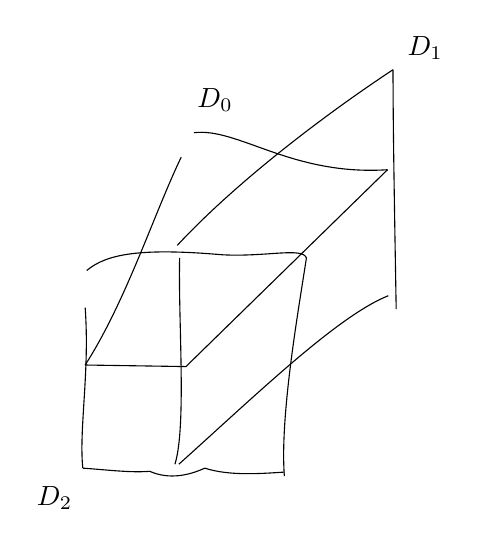
\begin{tikzpicture}[x=1cm,y=1cm]
\draw (0.05,0.12) .. controls (0.35,0.10) and (0.65,0.06) .. (0.90,0.08)
 .. controls (1.15,-0.03) and (1.40,0.03) .. (1.60,0.12);
\draw (1.60,0.12) .. controls (1.91,0.02) and (2.30,0.05) .. (2.61,0.07);
\draw (0.05,0.12) .. controls (0,0.62) and (0.14,1.35) .. (0.08,2.16);
\draw (2.61,0.02) .. controls (2.55,0.80) and (2.80,2.19) .. (2.89,2.79)
 .. controls (2.84,2.93) and (2.38,2.80) .. (1.82,2.83)
 .. controls (0.78,2.92) and (0.35,2.84) .. (0.10,2.63);
\draw (1.22,0.17) .. controls (1.37,0.65) and (1.26,2.03) .. (1.28,2.79);
\draw (1.25,2.95) .. controls (2.08,3.84) and (3.29,4.72) .. (3.99,5.18);
\draw (3.99,5.18) .. controls (3.99,4.40) and (4.01,3.34) .. (4.03,2.14);
\draw (1.27,0.17) .. controls (2.24,1.04) and (3.28,2.05) .. (3.93,2.31);
\draw (0.08,1.43) -- (1.36,1.41) -- (3.92,3.91);
\draw (0.08,1.43) .. controls (0.60,2.24) and (0.95,3.34) .. (1.30,4.07);
\draw (1.46,4.38) .. controls (2.02,4.45) and (2.70,3.83) .. (3.92,3.91);
\node[above] at (1.73,4.52) {$D_0$};
\node[above right] at (4.05,5.18) {$D_1$};
\node[below left] at (0.04,0.01) {$D_2$};
\end{tikzpicture}}

\figure{\begin{tikzpicture}
\begin{scope}[rotate=180,transform shape]
\node at (0,0) {$\mathbf T(\mathbf E_1,\ldots,\mathbf E_n)^{\deleted{\unsure{\Phi}}}$};
\node at (3.25,0.05) {$\deleted{\unsure{E}}\quad\mathcal F$};
\node at (-2.9,-0.67) {$\mathbf X$};
\node at (-1.70,-1.12) {$\mathbf K$};
\node at (-0.67,-0.63) {$\deleted{\unsure{\pi}}$};
\node at (-0.60,-0.92) {$p_1$};
\node at (0.55,-0.92) {$p_n$};
\node at (0.75,-2.03) {$\mathbf G_1\times\cdots\times\mathbf G_n$};
\node at (3.27,-1.99) {$\unsure{\mathcal K}$};
\end{scope}
\end{tikzpicture}}
\scanpage{106}
% archive foliation: 105
% Typescript is upside down relative to archive foliation.
\begin{center}- IV- \inserted{\unsure{878}} -\end{center}

\uline{un point de} $Y$.

Il résulte en effet de (17.4.1,(b'')) qu'une $Y$-section $s$ de $X$ est une immersion ouverte, et comme $X$ est un $Y$-schéma, $s$ est aussi une \deleted{\illegible{1}} immersion fermée (\uline{I},5.4.7); il en résulte que $s$ est un isomorphisme de $Y$ sur un sous-préschéma de $X$ induit sur une partie ouverte et fermée de $X$, et comme \deleted{\unsure{$X$}} $s(Y)$ est connexe, c'est nécessairement une composante connexe de $X$. Le reste de la proposition est immédiat.

\margin{\figure{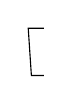
\begin{tikzpicture}\draw (0.20,0.6)--(0,0.6)--(0.04,0)--(0.2,0);\end{tikzpicture}}}
\uline{Proposition} (17.4.10) .- \uline{Soient} $g:Y\to S$, $h:X\to S$ \uline{deux morphismes localement de présentation finie. Pour qu'un} $S$-\uline{morphisme} $f:X\to Y$ \uline{soit non ramifié il faut et il suffit que pour tout} $s\in S$, \uline{le morphisme} $f_s:h^{-1}(s)\to g^{-1}(s)$ \uline{déduit de $f$ par le} \deleted{\illegible{1}} \uline{changement de base} $\operatorname{Spec}(\kappa(s))\to S$, \uline{soit non ramifié}.

Cela résulte aussitôt du fait que pour un morphisme localement de présentation finie, le fait d'être non ramifié est une propriété des \uline{fibres} de ce morphisme \inserted{(17.4.1,d))}, et \inserted{de ce} que pour tout $y\in Y$, on a $f^{-1}(y)=f_s^{-1}(y)$ si $s=g(y)$.
\margin{\figure{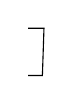
\begin{tikzpicture}\draw (0,0.6)--(0.2,0.6)--(0.18,0)--(0,0);\end{tikzpicture}}}

\uline{17.5. Caractérisations des morphismes lisses}.

\uline{Théorème} (17.5.1) .- \uline{Soient} $f:X\to Y$ \uline{un morphisme localement de présentation finie, $x$ un point de} $X$, $y=f(x)$. \uline{Les conditions suivantes sont équivalentes}:

a) \uline{$f$ est lisse au point $x$}.

\margin{\figure{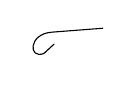
\begin{tikzpicture}[x=1cm,y=1cm]
\draw (1,.35)--(.35,.3) .. controls (.05,.28) and (.05,-.05) .. (.25,.03)--(.38,.15);
\end{tikzpicture}}}
b) \uline{$f$ est plat au point $x$ et le} $\kappa(y)$-\uline{préschéma} $f^{-1}(y)$ \uline{est lisse sur} $\kappa(y)$ \uline{au point $x$}.

b') \uline{$f$ est régulier au point $x$} (6.8.1).

c) \uline{L'anneau} $\mathrm O_{X,x}$ \uline{est une} $\mathrm O_{Y,y}$-\uline{algèbre formellement lisse pour les topologies discrètes}.

\margin{\figure{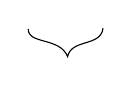
\begin{tikzpicture}[x=1cm,y=1cm]
\draw (0,.35) .. controls (0,.15) and (.4,.25) .. (.5,0) .. controls (.55,.23) and (.92,.12) .. (.95,.36);
\end{tikzpicture}}}
On peut se borner au cas où $Y=\operatorname{Spec}(A)$, \deleted{\unsure{$X=\operatorname{Spec}$}} $X=\operatorname{Spec}(C)$, où $C=B/\uline{J}$, $B=A[T_1,\ldots,T_n]$ étant une algèbre de polynômes et $\uline{J}$ un idéal de $B$ \uline{de type fini}. L'équivalence de a) et c) résulte alors de (\uline{0},22.6.4)\inserted{a)$\Leftrightarrow$c)}. D'autre part, comme $f^{-1}(y)$ est un $\kappa(y)$-préschéma localement \deleted{noethérien} \inserted{de type fini}, l'équivalence de b) et b') résulte de (6.8.6)\inserted{a)$\Leftrightarrow$b)}. Reste à voir que a) et b) sont équivalentes.

\margin{\diagram{\begin{tikzcd}[column sep=small]
{} \arrow[r,bend right] & \text{Attention à l'ambiguïté dans ``lisse'' !}
\end{tikzcd}}}
\scanpage{107}
% archive foliation: 106 (first digit partly clipped)
\figure{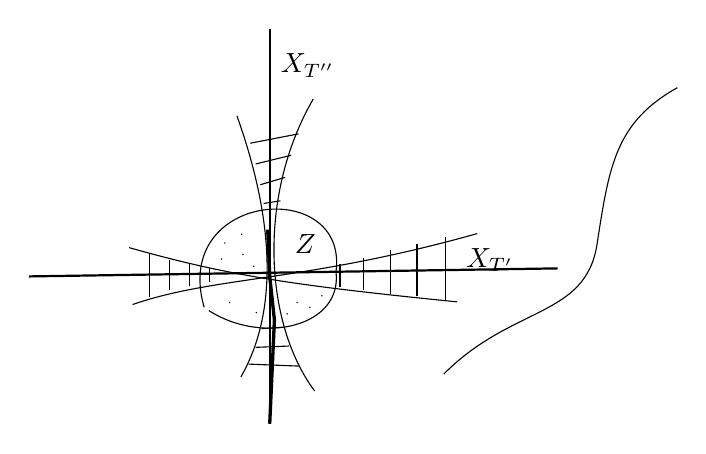
\begin{tikzpicture}[x=0.85cm,y=0.85cm]
\draw[thick] (-3.6,0)--(4.3,0.12);
\draw[thick] (0,-2.2)--(0,3.7);
\draw[very thick] (0,-2.2)--(0.07,-0.65)--(0,0)--(-0.03,0.7);
\draw (-2.1,0.43) .. controls (-0.65,0.02) and (0.3,-0.13) .. (2.8,-0.38);
\draw (-2.05,-0.42) .. controls (-0.8,0.01) and (0.5,-0.09) .. (3.1,0.64);
\draw (-0.49,2.40) .. controls (0.08,0.80) and (0.12,-0.54) .. (-0.43,-1.50);
\draw (0.65,2.65) .. controls (-0.18,1.22) and (-0.09,-0.69) .. (0.67,-1.71);
\draw (-0.29,1.99)--(0.43,2.13);
\draw (-0.21,1.68)--(0.32,1.81);
\draw (-0.14,1.37)--(0.23,1.48);
\draw (-0.09,1.09)--(0.16,1.13);
\draw (-0.12,-0.78)--(0.18,-0.76);
\draw (-0.21,-1.06)--(0.29,-1.04);
\draw (-0.32,-1.31)--(0.44,-1.34);
\foreach \x/\lo/\hi in {-1.8/-0.31/0.34,-1.5/-0.21/0.25,-1.2/-0.15/0.18,-0.9/-0.09/0.12,1.05/-0.16/0.18,1.4/-0.20/0.28,1.8/-0.26/0.39,2.2/-0.30/0.49,2.62/-0.36/0.59}{\draw (\x,\lo)--(\x,\hi);}
\draw (-0.98,-0.46) .. controls (-1.48,1.28) and (1.18,1.49) .. (0.99,0.07)
 .. controls (1.09,-0.75) and (-0.10,-1.03) .. (-0.91,-0.51);
\foreach \x/\y in {-0.67/0.50,-0.42/0.63,-0.72/0.26,-0.40/0.33,-0.24/0.15,-0.60/-0.39,-0.20/-0.54,0.26/-0.56,0.41/-0.39,0.60/-0.46,0.78/-0.29,0.54/0.62}{\fill (\x,\y) circle (0.012);}
\node at (0.53,0.48) {$Z$};
\node at (3.29,0.24) {$X_{T'}$};
\node[right] at (0.02,3.15) {$X_{T''}$};
\draw (2.6,-1.46) .. controls (3.62,-0.43) and (4.72,-0.62) .. (4.89,0.48)
 .. controls (5.07,1.64) and (5.16,2.30) .. (6.09,2.82);
\end{tikzpicture}}

\margin{$*$}
\diagram{\begin{tikzcd}[column sep=small,row sep=large]
\widehat{\mathbf Z}=\unsure{\Pi|\pi}_1(Z') \arrow[d] \arrow[drr] & & \unsure{\Pi|\pi}_1(Z'')=\widehat{\mathbf Z} \arrow[dl] \arrow[d] \\
\unsure{\Pi|\pi}_1(X_{T'}) \arrow[dr] & \unsure{\Pi|\pi}_1(X_{T''}) \arrow[d] & \unsure{\Pi|\pi}_1(Z)=\widehat{\mathbf Z}^{2} \arrow[dl] \\
& \unsure{\Pi|\pi}_1(X_T) &
\end{tikzcd}}

\figure{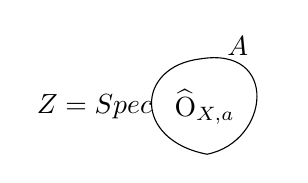
\begin{tikzpicture}
\node at (-1.4,0) {$Z=\operatorname{Spec}$};
\node at (0,0) {$\widehat{\mathrm O}_{X,a}$};
\draw (0.03,-0.60) .. controls (-0.91,-0.42) and (-0.88,0.51) .. (-0.06,0.61)
 .. controls (0.95,0.78) and (0.83,-0.44) .. (0.03,-0.60);
\node at (0.42,0.77) {$A$};
\end{tikzpicture}}
\[
X_{T'}\cap X_{T''}=\varnothing
\]
\[
X_{T'}\cap Z_{\deleted{\unsure{a}}}=Z'=\widehat A_{\unsure{p'|\mathfrak p'}}
\quad\begin{gathered}\unsure{correspond} -- \text{corps}\\
\text{résiduel }k(p')=\text{corps local en }a\text{ de }T'_0
\end{gathered}
\]
\[
X_{T''}\cap Z=Z''=\widehat A_{\unsure{p''|\mathfrak p''}}
\quad\begin{gathered}\unsure{correspond} -- \text{corps}\\
\text{résiduel }k(p'')=\text{corps local en }a\text{ de }T''_0
\end{gathered}
\]

On doit prouver un \uline{\unsure{th.} de descente} de nature essentiellement locale

$+$ déterminer certains \unsure{hom.} canoniques

\figure{\begin{tikzpicture}\draw (0,0)--(0.2,0.04);\draw (0.4,0.02)--(1.25,0.03);\draw (1.55,0.04)--(2.15,0.04);\end{tikzpicture}}

\margin{\diagram{\begin{tikzcd}[row sep=small]
\deleted{\unsure{A'}}\unsure{\}} \arrow[d,dash,bend right=30] \\
A \arrow[d] \\
B
\end{tikzcd}}}
\scanpage{108}
% archive foliation: 107
% Pale reversed typescript is mirror-image show-through from the other face.
\[
P=QQ'\qquad QR+Q'R'=1
\]
\margin{$(P)=(Q)(Q')=(Q)\cap(Q')$\par
car $s\in(Q)$, $s\in(Q')$\par
$\Longrightarrow s=Q'sR'+QsR\in(QQ')$}
\[
A[t]/(P)\longrightarrow A[t]/(Q)\times A[t]/(Q')
\]
injectif car $(\unsure{P})=(Q)\cap(Q')$

Surjectif car par Nakayama on est ramené au cas

$A[t]$

\uline{Lemme.} Soient $Q,Q'\subset A$ \uline{\unsure{id\textsuperscript{x}} étrangers}.

Alors $A/(QQ')\longrightarrow A/Q\times A/Q'$ est un \unsure{isom}.

En effet,\quad (i)\quad $(Q)\cap(Q')=QQ'$

car
\[
\underline Q\cap\underline {Q'}=\underline Q\cap\underline {Q'}(\underline Q+\underline {Q'})
\subset\underline {Q'}\underline Q+QQ'=QQ'.
\]
(ii) $\underline Q+\underline {Q'}=A$, \unsure{par hypothèse}; \unsure{il s'ensuit} que
\[
x\in A,\ y\in A\quad\Longrightarrow\quad
\begin{gathered}
\exists\unsure{b}\in Q\quad\text{qui est }\equiv y\quad(Q')\\
\exists a\in Q'\quad\text{qui est }\equiv x\quad(Q).
\end{gathered}
\]
donc
\[
a+b\equiv\begin{cases}x&(Q)\\y&(Q')\end{cases}
\]
\figure{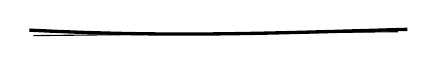
\begin{tikzpicture}\draw[very thick] (0,0) .. controls (1.8,-0.09) and (3.0,-0.04) .. (4.8,0.01);\draw (0.05,-0.07)--(4.68,-0.02);\end{tikzpicture}}

\diagram{\begin{tikzcd}[column sep=small,row sep=small]
A/Q.Q'\longrightarrow A/Q\unsure{\times|+}A/Q' & \text{surjectif }\deleted{\unsure{ssi}} \arrow[d,Leftrightarrow] & \\
& \text{bijectif} \arrow[d,Leftrightarrow] & \\
& Q+Q'=A \arrow[r,Rightarrow] & QQ'=Q\cap Q'
\end{tikzcd}}
\scanpage{109}
% archive foliation: 108
% Typescript is upside down relative to archive foliation.
\begin{center}Ad majorem fonctori gloriam\end{center}

J'apprends que Grothendieck n'est plus membre de Bourbaki. Je le regrette beaucoup, ainsi que les circonstances qui ont amené cette décision.

Il est bien entendu admis que Grothendieck n'aime pas la taquinerie ni le canular, tous deux chers à Bourbaki. Mais on se rode, et il était en bonne voie dans cette direction. D'autres y ont passé avant lui. De toute façon, ceci n'était qu'un côté secondaire de la question. Ce qui importait, c'est une opposition systématique, plus ou moins explicité selon les uns ou les autres, contre son point de vue mathématique, ou plutôt son emploie par Bourbaki.

Or, comme l'a très bien remarqué Kaplanski dans sa dernière review, Bourbaki n'est plus le youth impétueux qu'il était il y a vingt ans, mais une fixture moyenne-ageuse, ce qui est fort regrettable, mais malheureusement vrai.

C'est un scandale que Bourbaki, non seulement ne soit pas à la tête du mouvement fonctoriel, mais encore n'y soit même pas à la queue. Si Bourbaki tient à rester ce qu'il a voulu être, il est temps qu'il se réveille. Si certains membres fondateurs (e.g. Weil) désirent revenir sur leur décision de ne pas influencer Bourbaki dans la direction qu'il désire prendre, qu'ils le disent explicitement. A mon avis, c'est contraire aux habitudes de Bourbaki de trainer dans l'équivoque.

Comme suggestion pratique, je commence par proposer que Bourbaki adopte le livre de Grothendieck sur les catégories, ou toute autre variante, par exemple un fascicule de résultats extrait dudit livre.

Si Bourbaki refuse, non pas de se mettre dans le nouveau mouvement, mais d'en prendre la tête, alors les traités visant à la rédaction des éléments de mathématiques (et pas seulement à ceux de la géométrie algébrique) seront rédigés par d'autres, qui s'inspireront non pas de l'esprit de Bourbaki 1960, mais de son esprit 1936. Ce serait dommage.

\begin{center}-:-:-:-\end{center}

Je prends l'occasion pour indiquer une liste de questions catégoriques
\scanpage{110}
% archive foliation: 109
a) Donnons-nous un idéal $R\subset B$. Alors

Décomposition de $\unsure{B|A}/R$ en produit de deux anneaux
\[
\simeq\ \text{Donnée de deux idéaux }J,J'\text{ de }A\text{ tels que}
\]
\[
JJ'=R,\quad J+J'=A
\]
\margin{[Car $J+J'=A\Rightarrow JJ'=J\cap J'$]}

b) Supposons $B=A[T]$, \inserted{\figure{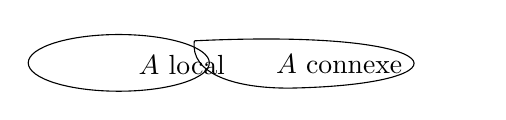
\begin{tikzpicture}
\node at (0,0) {\deleted{$A$ \uline{local}}};
\node at (2.0,0) {$A$ connexe};
\draw (-0.8,0.02) ellipse (1.15 and 0.36);
\draw (0.16,0.30) .. controls (3.5,0.46) and (3.75,-0.25) .. (1.40,-0.30)
 .. controls (0.68,-0.31) and (0.10,-0.12) .. (0.16,0.30);
\end{tikzpicture}}} $R=(P)$, $P$ polynôme \uline{unitaire}, Alors tte décomposition de $R$ en produit de deux idéaux $J,J'$ tels que $J+J'=B$, est \unsure{uniquement} de la forme $(\unsure{P|R})=(Q)(Q')$, où $Q,Q'$ sont des polynômes \uline{unitaires} tels que
\[
P=QQ'.
\]

Si elle est donnée par une telle déc., alors $P$ est unique à une unité près, et tt \unsure{repr.} unitaire est unique
\deleted{[\unsure{NB.}\quad\unsure{faut}}
[petite vérification\ldots]. \deleted{On}
\deleted{\unsure{prouver que}} \deleted{On}
\unsure{l'unicité résulte qu'} l'on peut supposer $\unsure{\operatorname{Spec}} A$ \uline{local}. Alors pour l'existence, on voit que c'est vrai sur les
\scanpage{111}
% archive foliation: 110
\deleted{\unsure{fatalité} par contre \unsure{ne} pourrait que m'inquiéter sérieusement}

\diagram{\(\begin{array}{ll}
A\ \text{anneau local }\deleted{\text{\unsure{intègre}}} & \widehat A\ \text{son complété}\\[1ex]
X=\operatorname{Spec}(A)&\widehat X\\[1ex]
D:\ \text{partie fermée}&\widehat D
\end{array}\)}

\figure{\begin{tikzpicture}[x=0.84cm,y=0.84cm]
% Left cutaway box, with dotted rear edge, curved sections, and marked points.
\draw (0.3,0.1) .. controls (0.6,0.02) and (1.2,0.0) .. (1.45,0.06);
\draw (0.3,0.1)--(0.37,1.54)--(1.7,1.48)--(1.65,0.13)--(2.3,0.77)--(2.34,2.06);
\draw (0.37,1.54)--(1.06,2.18)--(1.03,0.82);
\draw (1.2,2.19) .. controls (1.65,2.12) and (1.95,2.25) .. (2.25,2.19);
\draw (1.7,1.48)--(2.34,2.06);
\draw[dotted] (0.55,1.50)--(1.13,1.62)--(1.86,1.58);
\draw (0.36,0.72)--(1.78,0.72)--(2.37,1.33)--(2.30,1.68);
\draw (0.34,1.02)--(1.61,1.05);
\draw (0.35,0.87) .. controls (0.81,1.55) and (1.39,0.90) .. (1.65,0.13);
\draw (0.51,0.15) .. controls (0.65,0.40) and (0.85,0.56) .. (1.05,0.61);
\draw (1.66,0.13) .. controls (1.40,0.75) and (1.36,0.79) .. (1.44,1.08);
\fill (1.44,1.08) circle (0.045);
\draw (1.12,1.94) .. controls (1.57,2.00) and (1.58,1.69) .. (1.56,1.54);
\fill (1.56,1.54) circle (0.035);
\draw[->] (1.56,1.54)--(1.91,1.51);
\draw[->] (2.02,1.51)--(2.35,1.51);
\draw (1.94,1.47) .. controls (2.03,1.17) and (2.22,1.04) .. (2.33,0.97);
\draw (1.81,0.05)--(2.15,0.35);
% Central cutaway box with horizontal dark section and central marked point.
\draw (3.65,0.09)--(5.13,0.06)--(5.30,1.47)--(3.70,1.52)--(3.65,0.09);
\draw (3.56,1.58)--(4.37,2.37);
\draw (4.50,2.43)--(5.92,2.37)--(5.88,0.77)--(5.18,0.13);
\draw (5.30,1.47)--(5.92,2.37);
\draw[dashed] (4.39,2.25)--(4.31,0.77)--(5.88,0.77);
\draw[thick] (3.63,0.71)--(4.33,1.39)--(5.90,1.46)--(5.24,0.76)--(3.63,0.71);
\draw[very thick] (4.33,1.39)--(5.90,1.46)--(5.24,0.76);
\draw[dashed] (3.70,0.74)--(5.85,0.78);
\draw (4.65,1.57) .. controls (4.78,1.30) and (4.71,1.12) .. (4.72,1.03);
\fill (4.72,1.03) circle (0.10);
\draw (4.80,1.13) .. controls (5.35,1.10) and (5.36,1.11) .. (5.49,1.23);
\draw (3.73,0.15)--(3.91,0.13);
\draw (5.59,1.72)--(5.92,2.37);
% Small marked surface and adjoining lettering.
\draw (7.45,1.48) .. controls (7.78,1.73) and (7.77,2.02) .. (7.85,2.21)
 .. controls (8.15,2.16) and (8.44,2.22) .. (8.62,2.22)
 .. controls (8.55,1.85) and (8.41,1.63) .. (8.28,1.47)
 .. controls (7.92,1.40) and (7.66,1.42) .. (7.45,1.48);
\fill (8.07,1.87) circle (0.085);
\node at (10.63,1.30) {$\mathbf Z\quad\deleted{\unsure{f_x}}$};
\node at (9.46,0.70) {$\mathbf x$};
% Labels and diagrams below the sketches.
\node[anchor=north west,inner sep=0] at (1.86,-0.68) {\begin{minipage}{2cm}\unsure{\diagram{\begin{tikzcd}[ampersand replacement=\&,column sep=small]\widehat Y\arrow[r]\&\widehat Z\end{tikzcd}}}\end{minipage}};
\node at (5.47,-1.03) {$\widehat Y\times_{\widehat S}\widehat Z$};
\node at (8.31,-1.03) {\deleted{\unsure{connexe}}};
\node at (2.33,-2.05) {$Y\times Z$};
\node[anchor=north west,inner sep=0] at (3.49,-1.76) {\begin{minipage}{5cm}\diagram{\begin{tikzcd}[ampersand replacement=\&,row sep=small]H\ \text{composante connexe}\arrow[d]\\Y\times Z\end{tikzcd}}\end{minipage}};
% Completion square with literal unheaded lower connectors.
\node[anchor=north west,inner sep=0] at (8.1,-3.05) {\begin{minipage}{5.6cm}\diagram{\begin{tikzcd}[ampersand replacement=\&,column sep=small,row sep=small]
S\&\widehat S\arrow[l]\\
X\arrow[u]\&\widehat X\arrow[l]\arrow[u]\\
\deleted{\unsure{Y}}A\arrow[u]\arrow[r,dash]\&A'\arrow[u]\arrow[r,dash]\&\widehat A=\unsure{\widehat{A'}|A'}
\end{tikzcd}}\end{minipage}};
% Long surrounding stroke and lower-left brace-like contour.
\draw (0.05,2.55) .. controls (-0.10,2.75) and (3.2,2.71) .. (7.8,2.92)
 .. controls (10.5,3.05) and (12.6,3.45) .. (12.58,1.80)
 .. controls (12.63,0.22) and (12.12,-0.08) .. (10.98,-0.23)
 .. controls (9.65,-0.41) and (8.93,-1.61) .. (8.88,-2.24)
 .. controls (8.77,-3.04) and (10.70,-2.36) .. (11.56,-2.51)
 .. controls (12.10,-2.55) and (11.54,-3.46) .. (12.24,-4.40)
 .. controls (12.72,-5.15) and (13.27,-5.84) .. (13.47,-5.92);
\draw (0.17,-1.12) .. controls (0.14,-2.77) and (0.13,-2.94) .. (3.68,-3.17);
\draw (-0.16,-3.62) .. controls (0.87,-3.24) and (2.69,-3.29) .. (3.74,-3.35)
 .. controls (4.55,-3.43) and (4.21,-5.53) .. (4.35,-6.12);
\draw (0.07,-6.04) .. controls (1.62,-6.10) and (1.11,-5.75) .. (1.02,-4.95)
 .. controls (0.77,-3.67) and (3.37,-3.84) .. (3.20,-4.96)
 .. controls (3.13,-5.54) and (2.23,-6.21) .. (2.94,-6.22)--(3.98,-6.22);
\draw (4.57,-3.28) .. controls (5.58,-3.15) and (4.88,-6.51) .. (5.55,-7.52);
\draw (6.06,-3.11) .. controls (4.82,-3.00) and (5.03,-4.73) .. (6.14,-4.07)
 .. controls (6.94,-3.60) and (6.45,-3.07) .. (6.06,-3.11);
% Lower pen sketches: crossing arcs, starbursts, and isolated heavy strokes.
\draw[thick] (5.81,-6.89) .. controls (6.59,-6.52) and (7.03,-6.43) .. (7.75,-6.51);
\draw (6.86,-5.98)--(6.79,-7.44);\draw[thick] (6.58,-6.21)--(7.08,-6.96);\draw (7.14,-6.06)--(6.64,-6.92);
\draw (7.30,-8.08) .. controls (7.45,-7.40) and (7.26,-7.29) .. (7.56,-6.99);
\draw (7.25,-7.31)--(7.68,-7.89);
\draw (7.91,-6.81) .. controls (7.76,-6.17) and (8.10,-5.67) .. (8.28,-5.34);
\draw (7.90,-5.37)--(8.32,-6.19);
\draw (8.42,-7.50) .. controls (9.01,-6.81) and (9.20,-6.74) .. (9.81,-6.54);
\draw (8.97,-5.74) .. controls (8.86,-6.46) and (9.11,-7.33) .. (9.42,-7.70);
\fill (9.10,-6.87) circle (0.04);
\draw[thick] (10.12,-6.13) .. controls (10.31,-6.83) and (10.23,-7.24) .. (10.38,-7.55);
\draw (10.57,-6.13)--(10.13,-7.27);\draw[thick] (10.29,-6.79)--(10.57,-7.10);
\draw[thick] (11.34,-6.86)--(11.58,-7.46);\draw (11.10,-7.36)--(11.72,-7.05);\draw (11.19,-7.06)--(11.73,-7.25);\draw (11.57,-6.99)--(11.20,-7.48);
\draw[line width=2pt] (11.72,-6.02)--(12.12,-6.41);\draw[line width=2pt] (13.00,-5.92)--(13.47,-6.32);
\end{tikzpicture}}
\scanpage{112}
% archive foliation: 111
\begin{flushright}Notes pour SGA 7\end{flushright}
\scanpage{117}
% archive foliation: 116
Comportement fonctoriel des groupes d'inertie.

1. Soient $X$ un schéma, $U$ un ouvert de $X$, $G$ un groupe profini, $U'$ un revêtement principal de $U$ de groupe $G^{\deleted{\unsure{'}}}$, $x$ un point \inserted{géom.} de $X$, $\overline X$ le localisé strict de $X$ en $x$, $\overline U$ l'image inverse de $U$ dans $\overline X$, $\overline U'=U'\times_U\overline U$. On suppose donné de plus un schéma $\overline X'$ sur $\overline X$, avec des opérations de $G$ sur $\overline X'$, de telle façon que le \deleted{espace} \inserted{$\overline U$-schéma} à opérateurs $\overline X'|\overline U$ coïncide avec $\overline U'$.

Pratiquement, on sera intéressé par le cas où $x\in X-U$ et où $x$ est adhérent à $U$, où $\overline X'$ est entier sur $\overline X$ et où $\underline{\mathrm O}_{\overline X}=\overline p(\underline{\mathrm O}_{\overline X'})^G$, $\overline p:\overline X'\to\overline X$ étant la projection canonique, - de sorte que $G$ opère transitiv\deleted{\unsure{e}}ement sur l'ensemble fibre $\overline X'_{\overline x}$. De plus, on \deleted{\unsure{se placera}} sera \inserted{le plus souvent,} sous des conditions où on peut construire canoniquement $\overline X'$ en termes de $\overline U'$; par exemple, si on suppose $X$ normal en $x$, donc $\overline X^{\deleted{\unsure{'}}}$ normal, et $\overline U$ non vide, on définira $\overline X'$ comme le normalisé de $\overline U$ relativement à $\overline U'$ sur $\overline U$ (i.e. comme limite projective des \unsure{normaalisés|normalisés} dans les $\overline{U'(i)}$ sur $\overline U$, $U'$ étant écrit comme limite projective de schémas principaux $U'(i)$ sur les groupes quotients finis $G(i)$ de $G$).

Si maintenant \deleted{\unsure{$X$} est} \inserted{$\xi$} est un point de $\overline X'_{\overline x}$, on peut considérer le groupe de stabilité $G_\xi$ de $\xi$, formé des $g\in G$ tels que $g.\xi=\xi$; ce groupe prendra le nom de \uline{groupe d'inertie} \uline{relatif à} $\xi$. Dans le cas envisagé plus haut où les points de $\overline X'$ sur $\overline x$ sont tous conjugués sous $G$, on voit que pour $\xi$ variable\deleted{\unsure{s}}, les $G_\xi$ parcourent une classe de sous-groupes conjugués de $G$, qu'on appellera \inserted{(par abus de langage)} \uline{les sous-groupes d'inertie} \deleted{de} \uline{relatifs à} $x$. Noter qu'en toute rigueur cette classe de sous-groupes \deleted{d'inertie} n'est pas déterminée par la seule connaissance de $x\in X$, mais dépend du choix du prolongement de $\overline U'$ en $\overline X'$. Lorsque $X$ est normal en $x$ et que $x$ est spécialisation d'un point de $U$ (ce qui signifie que $x$ est adhérent à $U$ si $\operatorname{esp}(X)$ est localement noethérien), il sera sous-entendu, sauf mention du contraire, que le choix en question est fait par normalisation, comme expliqué plus haut.
\scanpage{118}
% archive foliation: 117
% The reversed pale body text is show-through of scan 117.
% The cancelled typescript fragment below is upside down on this face.
\deleted{(2.1.14.6)
\diagram{\(\begin{array}{ccc}
P&\unsure{\otimes}&Q\\
\underline a&&\underline b
\end{array}\)}}
\figure{\begin{tikzpicture}\draw[line width=0.8pt] (0,0.20) .. controls (0.02,0.12) and (0.04,0.05) .. (0.05,0);\end{tikzpicture}}
\scanpage{124}
% archive foliation: 123
\begin{flushright}
``\uline{Vrai}'' groupe\\
fondamental

[pour les\\
\unsure{ensembles|schémas}]
\end{flushright}
\scanpage{126}
\mspage{2}
% archive foliation: 125
 de schémas en groupes finis et plats sur $S$
\diagram{\begin{tikzcd}[column sep=small]
e \arrow[r] & H_{\mathrm{inf}} \arrow[r] & H \arrow[r] & H_{\text{sép}} \arrow[r] & e
\end{tikzcd}}
où $H_{\mathrm{inf}}$ est purement infinitésimal (i.e. la projection $H_{\mathrm{inf}}\to S$ est géométriquement injectif) et où $H_{\text{sép}}$ est non ramifié sur $S$. (Dans le cas d'un corps de base $k$, une telle suite exacte est déduite d'une suite exacte analogue pour un groupe algébrique fini \inserted{$G$} sur $k$; d'ailleurs si $k$ est parfait, cette suite splitte canoniquement, car $G_{\text{réd}}$ est \inserted{alors} un sous-groupe de $G$, isomorphe à $G_{\text{sép}}$ par la projection $G\quad G_{\text{sép}}$. Faire attention cependant que $G_{\text{réd}}$ va opérer sur $G_{\mathrm{inf}}$, on aura seulement un produit semi-direct). Enfin

\deleted{La condition (v) \unsure{est essentiellement provisoire}.}

(vi) $S$ est réduit.

Les conditions (v) et (vi) ont une sale gueule, et sont essentiellement provisoires. Elles servent à \deleted{\unsure{justifier la vérité}} \inserted{\unsure{cause}} du

\uline{Lemme}. Soit $H$ comme dans (v), $S$ comme dans (vi), $P$ un fibré principal homogène sous $H$, $Q$ un autre, $u,v$ deux isomorphismes de $P$ dans $Q$ transformant un \inserted{``}point \deleted{\unsure{géométrique}} \inserted{marqué''} donné en un autre donné, alors $u=v$. (On est ramené, en tordant $H$, au cas où $P$ est trivial, et alors cela résulte du fait suivant: une section de $Q$ est un isomorphisme de $S$ sur une composante connexe de $Q_{\text{réd}}$).

Remarque néanmoins que les conditions (i) à (vi) n'excluent pas des groupes structuraux tordus (relativement à un corps de base $k$).

Soit maintenant $a$ un ``point marqué'' de $S$ (i.e. une extension algébriquement close du corps résiduel d'un $s\in S$). Pour tout $G\in\underline G$, on désigne par $Z(S,a;G)$ ou simplement $Z(G)$ l'ensemble des classes (à isomorphisme près) de fibrés principaux homogènes sur $S$, de groupe $F(G)$, munis d'un point marqué au dessus de $a$. Evidemment $Z(G)$ est un foncteur de $\underline G$ dans la catégorie des ensembles. Ce foncteur satisfait aux conditions suivantes: 1) Il commute aux produits (\deleted{trivial) \unsure{et}} car $F$ y commute) 2) il commute aux noyaux de couples, en d'autres termes si
\diagram{\begin{tikzcd}[column sep=small]
G'' \arrow[r] & G \arrow[r,shift left=.6ex] \arrow[r,shift right=.6ex] & G'
\end{tikzcd}}
est exact dans $\underline G$, alors
\diagram{\begin{tikzcd}[column sep=small]
Z(G'') \arrow[r] & Z(G) \arrow[r,shift left=.6ex] \arrow[r,shift right=.6ex] & Z(G')
\end{tikzcd}}
est exacte, i.e. $Z(G'')$ s'identifie à l'ensemble des éléments de $Z(G)$ dont l'image dans $Z(G')$ par $Z(u)$ et $Z(v)$ est la même. (Ceci résulte de l'exactitude de $F$, et du lemme).
\figure{
\begin{tikzpicture}[scale=.4]
\draw[line width=.6pt] (0,.1)--(.08,.32)--(.22,.35)--(.4,.53)--(.13,.42)--(.04,.3)--(.1,-.1)--(.21,-.22)--(.41,-.14)--(.23,-.3)--(.12,-.1)--(-.03,.17)--(.22,.23);
\end{tikzpicture}}
\scanpage{129}
\mspage{5}
% archive foliation: 128
Lorsqu'il n'y a pas de corps de base, il n'est pas clair cependant comment et à quels groupes fondamentaux \deleted{\unsure{respectifs}} pour $X,Y$ on peut rattacher \deleted{par une suite} les groupes fondamentaux des fibres, pour tenir lieu de suite exacte d'homotopie. S'il y a un corps de base, une \deleted{hypothèse} \inserted{conjecture} de départ serait que \deleted{l'image inverse par $f$ de} $\underline\Pi_1(X/Y)$, le pro-schéma en groupes \inserted{$\underline\Pi_1(X)$} sur $X$ qui définit le système local des groupes fondamentaux \deleted{\unsure{en $x$}} de $X$ en ses divers points, et enfin l'image inverse par $f$ du pro-schéma en groupes analogue \inserted{$\underline\Pi_1(Y)$} sur $Y$, sont reliés par une suite exacte \deleted{(qui serait définie d'ailleurs indépendamment de l'existence d'une section de $X$ sur $Y$, car le premier \deleted{\unsure{groupe}} pro-schéma en groupes \inserted{(sur $X$,} nommé serait défini en tous cas). Si $Y$ est le spectre d'un anneau local complet, notamment un anneau de valuation discrète, on devrait pouvoir \unsure{mettre}} il y a de la joie en perspective pour les groupes d'homotopie supérieurs\ldots

Il n'est pas dit que la conjecture envisagée soit plus difficile à démontrer que la partie déjà connue pour les groupes fondamentaux ordinaires. Elle impliquerait que pour des schémas complets $X,Y$ au dessus d'un corps alg clos $k$, on a $\Pi_1(X\times Y/k)=\Pi_1(X/k)\times\Pi_1(Y/k)$. Utilisant tes raisonnements, on en conclut que si $X$ est une variété abélienne sur $k$, alors $\Pi_1(X/k)$ est abélien, et qu'un revêtement principal minimal $X'$ de $X$ est une variété abélienne isogène à $X$. On en déduit
\[
\Pi_1(X/k)=\varprojlim {}_nX
\]
où ${}_nX$ est le noyau (avec sa partie infinitésimale aussi, bien sûr) de la multiplication par $n$, l'homomorphisme de ${}_{mn}X$ dans ${}_nX$ étant induit par la multiplication par $m$. (Utilisant Cartier, ce groupe fondamental est dual, au sens de Cartier, au groupe ind-algébrique limite inductive des ${}_nX^*$, où $X^*$ est la variété duale de $X$). Prenant la $p$-composante de ce groupe fondamental, on trouve ce qui, pour le nombre premier $p$, doit jouer le rôle du module de Weil. Il est hors de doute (et Cartier doit l'avoir fait) qu'il est possible d'associer \deleted{\unsure{à un}} fonctoriellement à un groupe proalgébrique infinitésimal abélien un module sur l'anneau de Witt, et \deleted{\unsure{donc}} qu'il \inserted{\unsure{soit|est}} facile de vérifier qu'en l'occurrence ce module se décompose en les trois morceaux que tu connais bien (correspondants aux trois types principaux de \inserted{$p$-}groupes algébriques abéliens), \deleted{qui} On trouve ainsi
\scanpage{130}
\mspage{6}
% archive foliation: 129
pour ton théorème une formulation plus naturelle (qui devrait \deleted{\unsure{en}} fournir une démonstration uniforme, sans distinction du cas $\ell\ne p$ et $\ell=p$), de même qu'on voit en même temps que ta somme abracadabrante se comporte bien quand on fait varier $X$ dans une famille, i.e si $X$ est \deleted{en fait un} un schéma abélien sur $Y$ (car alors les ${}_nX$ seront d'excellents schémas en groupes finis et plats sur $Y$, dont on peut prendre formellement la limite projective\ldots).

J'espère \unsure{arriver-dans|arriver dans} l'année prochaine à une théorie satisfaisante du groupe fondamental, \deleted{\unsure{ce qui}} et achever la rédaction des Chapitres IV,V,VI,VII (ce dernier étant le groupe fondamental), en même temps que des catégories. Dans deux ans résidus, dualité, intersections, Chern, Riemann-Roch. Dans trois ans cohomologie de Weil, et un peu d'homotopie si Dieu veut. Et entre-temps, je ne sais quand, le grand théorème d'existence avec Picard etc, un peu de courbes algébriques, \inserted{les schémas abéliens.} Sauf difficultés imprévues ou enlisement, le multiplodoque devrait être fini d'ici 3 ans, ou 4 au maximum. On pourra commencer à faire de la géométrie algébrique !

Bien à toi
\scanpage{131}
% archive foliation: 130
\diagram{\begin{tikzcd}X\arrow[d,"f"]\\S\end{tikzcd}}
muni d'une section $\sigma$, $f$ propre plat, $f_*\mathcal O_X=\mathcal O_S$ \uline{\unsure{universellt|universelle}}.

$G$ schéma en groupes \deleted{\unsure{plat}} fini et \deleted{\unsure{séparable}} \inserted{étale} sur $S$ [le cas important est celui où $G=S\times\Gamma$].

$F_G(T)=$ ens des classes à isom. près des fibrés principaux homogènes sur $X_T$, de groupe
\[
G_T\times_T X_T=(G\times_S X)_T\deleted{\unsure{\times X}},
\]
\uline{munis} d'une section marquée le long de $\sigma_T$, i.e. \inserted{d'un isom.} $\sigma_T^*(X')\simeq G_T$.

N.B. Tout automorphisme d'un tel \unsure{fibré|fonct.} est trivial, \unsure{puisqu'on suppose que} $G$ est \deleted{\unsure{inf}} étale sur $S$. Il en serait de $=$ pour $G$ commutatif. \unsure{Cas fini}??

Le foncteur $F_G(T)$ en $T$ est-il représentable?? Si oui, le \unsure{sch.} sur $S$ qui le représente est \uline{étale} sur $S$, et \uline{quasi-fini sur $S$} [cas à fibres \uline{finies}].

Noter que le foncteur $F_G$ est \deleted{\unsure{compatible}} \unsure{ex. et à gauche} pour les morphismes fid. plats et quasi-compacts.

\margin{\figure{\begin{tikzpicture}[scale=.58,rotate=180,transform shape]
\node at (0,5.4) {\begin{minipage}{9cm}\diagram{\begin{tikzcd}[ampersand replacement=\&,column sep=small,row sep=large]
C \arrow[r,very thick] \arrow[d,no head] \& C' \arrow[r,shift left=.6ex] \arrow[r,shift right=.6ex] \arrow[d,very thick] \& C'' \arrow[r,shift left=1.2ex] \arrow[r] \arrow[r,shift right=1.2ex,no head] \arrow[d,no head] \& C^{\prime\prime\prime} \arrow[d,no head] \\
C_{\unsure{\bullet}} \arrow[r,no head] \& C'_{\unsure{\bullet}} \arrow[r,shift left=.6ex] \arrow[r,shift right=.6ex] \& C''_{\unsure{\bullet}} \arrow[r,shift left=1.2ex] \arrow[r] \arrow[r,shift right=1.2ex,no head] \& C^{\prime\prime\prime}_{\unsure{0}}
\end{tikzcd}}\end{minipage}};
\node at (-3.8,4.8) {\uuline{\unsure{finis?}}};
\fill (-2.3,3.9) circle (.055); \fill (-.8,3.9) circle (.055);
\node at (-.7,3.45) {\uline{\unsure{fid. plat}}};
\node at (2.0,3.45) {\uline{plat}};
\draw (-1.3,2.8) .. controls (0,3.0) and (1.5,3.2) .. (2.4,2.7) .. controls (3.3,3.0) and (4,2.9) .. (4.6,3.3);
\node at (2.5,2.3) {\unsure{exacte}};
\node at (.1,-.9) {4.9.};
\node at (3.2,-.9) {\unsure{4.17.|4.13.}};
\node at (1.2,-4.3) {4.9.};
\draw (-3.2,6.6) .. controls (-1,6.4) and (1.7,6.3) .. (2.5,6.2) .. controls (2.9,5) and (2.5,0) .. (2.5,-3.8) .. controls (2.5,-4.6) and (1.4,-4.7) .. (.1,-4.6);
\draw (-1.5,6.8)--(2.0,-4.5);
\draw (-4,5.1) .. controls (-3,1) and (-1.1,-2.4) .. (-.5,-4.1);
\fill (-.5,6.9) circle (.045);
\end{tikzpicture}}}

\figure{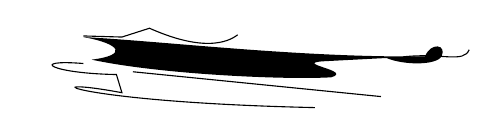
\begin{tikzpicture}[x=.7cm,y=.7cm]
\draw (0,.6)--(.7,.58)--(1.2,.74) .. controls (2.3,.25) and (2.7,.55) .. (2.8,.62);
\fill (0,.58) .. controls (.7,.45) and (.8,.25) .. (.15,.17) .. controls (1.4,-.1) and (3.7,-.2) .. (4.5,-.15) .. controls (4.9,-.03) and (3.8,.1) .. (4.35,.14) --(5.5,.2) .. controls (5.8,.07) and (6.4,.06) .. (6.5,.23) .. controls (6.6,.45) and (6.3,.49) .. (6.2,.23) .. controls (4,.2) and (1.5,.5) .. (0,.58);
\draw (0,.1) .. controls (-1,.18) and (-.6,-.08) .. (.6,-.1)--(.7,-.43) .. controls (-1,-.11) and (-.3,-.6) .. (4.2,-.7);
\draw (.9,-.05)--(5.4,-.5); \draw (5.8,.22) .. controls (6.5,.3) and (6.9,.1) .. (7,.35);
\end{tikzpicture}}

\figure{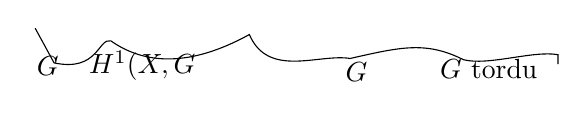
\begin{tikzpicture}[x=.8cm,y=.8cm]
\node at (0,0) {$\deleted{\unsure{G}}$};
\node at (1.5,0) {$H^1(X,G$};
\node at (4.9,-.1) {$G$};
\node at (7,-.05) {$G$ \uline{tordu}};
\draw (-.2,.6)--(.1,.05) .. controls (.8,-.1) and (.8,.45) .. (1,.4) .. controls (1.5,.05) and (2.2,-.05) .. (3.2,.5) .. controls (3.5,-.2) and (4.3,.2) .. (4.8,.12) .. controls (5.6,.3) and (6,.4) .. (6.6,.1) .. controls (7,0) and (7.7,.25) .. (8.1,.18)--(8.1,.03);
\end{tikzpicture}}
\scanpage{132}
% archive foliation: 131
% Typescript is upside down in the supplied scan; read in its own orientation.
I-6

subset of $\underline L$ consisting of the maps rational over $k$. The correspondence $f\longrightarrow(f^j_{\unsure{\alpha|a}_1,\ldots,\unsure{\alpha|a}_r})$ is linear and one-to-one between $\underline L$ and the set all families of elements in $K$ with only a finite number of nonzero components; since $\underline L_k$ is mapped in this way on the set of all families with components in $k$, one sees that $\underline L_k$ is a $k$-structure on $\underline L$. Furthermore, for any field $k'$, the set $\underline L_{k'}$ of the multilinear maps rational over $k'$ is equal to $k'.\underline L_k$.

Let finally $V$ and $W$ be two vector spaces with respective $k$-structures $V_k$ and $W_k$, and let $f$ be a linear map from $V$ to $W$ rational over $k$. If a subspace $S$ of $V$ is rational over $k$, it is generated by $S\cap V_k$ and therefore $f(S)$, being generated by $f(S\cap V_k)\subset W_k$, is rational over $k$. Let now $T$ be a subspace of $W$ rational over $k$; for a $k$-basis $\{c_{\unsure{\alpha|a}}\}$ of $K$, any vector $v$ in $V$ is uniquely expressed as $\sum_{\unsure{\alpha|a}} c_{\unsure{\alpha|a}}.v_{\unsure{\alpha|a}}$ for some $v_{\unsure{\alpha|a}}$ in $V_k$, and such a vector is in $T$ if and only if $f(v_{\unsure{\alpha|a}})$ is in $T$ for all $\unsure{\alpha|a}$ since $f(v)=\sum_{\unsure{\alpha|a}}c_{\unsure{\alpha|a}}.f(v_{\unsure{\alpha|a}})$; therefore $f^{-1}(T)$ is generated by $f^{-1}(T)\cap V_k$ and is rational over $k$.

From the previous results, we shall deduce that the linear map $f$ is rational over $k$ if and only if its graph $\Gamma$ is a subspace of $V\times W$ rational over $k$ (for the $k$-structure $V_k\times W_k$ on $V\times W$). Indeed, $\Gamma$ is the image of the map $g:v\longrightarrow(v,f(v))$ of $V$ into $V\times W$ and if $f$ is rational over $k$, so is $g$ and so is its image $\Gamma$. Conversely, assume $\Gamma$ rational over $k$; there exists therefore a basis of $\Gamma$ consisting of vectors of $V\times W$ rational over $k$; such a basis is of the form $\{(e_i,f(e_i))\}$ where $e_i$ and $f(e_i)$ are rational over $k$ for all $i$; but since the projection from $\Gamma$ to $V$ is an isomorphism of vector spaces, the $e_i$ form a basis of $V$ rational over $k$, and since the $f(e_i)$ are rational over $k$, so is $f$.

5. \uline{Conjugates}.

\uline{Let} $V$ \uline{be a vector space with a $k$-structure} $V_k$ \uline{and let} $\sigma$ \uline{be a $k$-isomorphism from a field} $k'$ \uline{onto a field} $k''$.

We shall study the behavior under $\sigma$ of the vectors, the subspaces and the multilinear maps. To begin with, I contend that there exists a unique map $v\longrightarrow v^\sigma$ from $V_{k'}$ onto $V_{k''}$ such that:
\scanpage{133}
% archive foliation: 132
\deleted{\unsure{(iv)}}

$S$ préschém. loc. noeth.

$F$ foncteur
\diagram{\begin{tikzcd}(\text{Sch})_{/S}\arrow[r] & (\text{Ens})\end{tikzcd}}

(i) $F$ compatible aux limites inductives d'anneaux

(ii) $F$ compatible aux descentes \unsure{fidèlement} plats qua. cpts. \inserted{et localisation}

[(iii) Si $A$ anneau local noeth. \uline{complet} sur $S$, corps résiduel $k$, alors $F(A)\xrightarrow{\sim}F(k)$,

(iv) $F$ séparé.

(v) Pour \unsure{tt} corps $k$ sur $S$, $F(k)$ est \uline{fini}, et si $K'$ est une ext. alg. close de $k$, \deleted{\unsure{plat|$k$}} alg. clos, $F(k)\unsure{-|\to}F(k')$ est bijectif.

Alors $F$ représentable par un \deleted{foncteur} objet étale \deleted{et qu.} séparé qu. fini sur $S$.

\deleted{\unsure{Recommençons}}

Supposons $S$ le spectre d'un anneau local complet $A$, \inserted{à corps résiduel alg. clos.} \deleted{et que} de dim $\unsure{n|1}$, et qu'on sache que sur $S_1=S-\unsure{y|s}$, le foncteur $F$ soit représentable par $M_1$. \deleted{Considérons les \unsure{points}} Soient $\xi_i^0\deleted{\unsure{\in F_0/k}}$ \inserted{$(i\in I)$}, éléments de $F(k)$, ils proviennent d'éléments $\xi_i\in F(A)$ bien déterminés, considérons leurs restrictions $\xi_i'=\xi_i|S_1\in F(S_1)$, ils correspondent à des
\scanpage{135}
% archive foliation: 134
\uline{Lemme} Soit $S$ un préschém. loc noeth., et pour \unsure{tout|tt} $s\in S$, soit $\deleted{\unsure{X_s}}$ $X(s)$ un préschém. quasi fini \uline{étale} \uline{séparé} sur $\operatorname{Spec}(\mathcal O_s)$, et pour $t\in S$, $s\in\overline t$, soit $\varphi_{st}:X(t)\unsure{-|\to}X(s)$ rendant cartésien le diagramme ci-contre.
\diagram{\begin{tikzcd}[column sep=large]
X(s) \arrow[d] & X(t) \arrow[l] \arrow[d] \\
\operatorname{Spec}(\mathcal O_s) & \operatorname{Spec}(\mathcal O_t) \arrow[l]
\end{tikzcd}}
On suppose que $\varphi_{ss}=\text{identité}$
\[
\varphi_{st}\varphi_{tu}=\varphi_{su}.
\]
\deleted{\unsure{des}}
\inserted{[On suppose que pour tt $s\in S$, il existe \unsure{une définition de} \deleted{\unsure{la}} $\mathcal X$ de $X(s)$ sur un voisinage ouvert $U$ de $s$, \deleted{\unsure{le groupe}} pour tt $t\in U$, un hom \deleted{$\unsure{X_t}$} $\mathcal X\times_U\operatorname{Spec}(\mathcal O_t)\to X(t)$, ces hom étant compatibles avec les \unsure{$\varphi$}.]}
\diagram{\begin{tikzcd}[column sep=small,font=\small]
X(s) \arrow[r,no head] \arrow[d] & \mathcal X \arrow[d] & \mathcal X\times_U\operatorname{Spec}(\mathcal O_t) \arrow[l] \arrow[r] \arrow[d] & X(t) \\
\operatorname{Spec}(\mathcal O_s) \arrow[r] & U & \operatorname{Spec}(\mathcal O_t) \arrow[l] &
\end{tikzcd}}
Alors il existe un préschém. étale \inserted{quasi-fini séparé} sur $S$, soit $X$, et des \inserted{$\mathcal O_s$-}isom
\[
\varphi_s:X\times_S\operatorname{Spec}(\mathcal O_s)\unsure{-|\to}X(s)
\]
rendant commutatifs les diagrammes qu'on pense. $X$ est unique à isom unique près.

Ce dernier fait résulte d'un énoncé plus général sur les catégories des préschémas de type fini sur $S$, qui donne un foncteur pleinement fidèle. \unsure{Je vais pour du moins ramener au local} et supposer $S$ affine, donc noeth. \unsure{le prouver} par récurrence noethérienne, en supposant l'énoncé prouvé pour les sous-préschémas fermés de $S\ne S$.
\scanpage{137}
% archive foliation: 136
Soit $S$ un schéma \uline{réduit} \uline{connexe}.

On considère des schémas en groupes, finis et plats sur $S$, soit $G$, pour lesquels on a une suite exacte
\diagram{\begin{tikzcd}[column sep=small]
e \arrow[r,no head] & \unsure{U|H} \arrow[r] & G \arrow[r,no head] & \Gamma \arrow[r] & e
\end{tikzcd}}
où la projection $U\to S$ est plate, finie, \deleted{\unsure{s}} et géométriquement \deleted{\unsure{un homéomorphisme}} injectif, et où $\Gamma\unsure{-|\to}S$ est plat, fini, séparable. Alors le sous-$S$-groupe $U$ de $G$ est déterminé de façon unique [pour cette assertion, l'hypothèse ``$S$ réduit'' est-elle nécessaire?].
\margin{\uline{$S$-Groupes} \uline{admissibles} ($S$ réduit?)}
On veut étudier des fibrés principaux \inserted{hom.} $P$ sur de tels $S$-groupes. On suppose $S$ pointé par $a\deleted{\unsure{\xi}}$, et on considère des $P$ avec structure pointée.

\margin{\figure{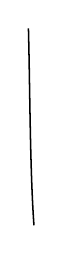
\begin{tikzpicture}\draw[line width=.55pt] (0,2.5) .. controls (.02,1.7) and (.02,.7) .. (.07,0);\end{tikzpicture}}}
\uline{Proposition} \deleted{\unsure{soit $S'\to S$}} Soit $S'\to S$ un morphisme \deleted{plat fini surjectif fidèlement plat}, $G$ un $S$-groupe fini. \deleted{Si $G\times_S S'$ est admissible,} \unsure{?} \inserted{Si $G\deleted{\unsure{\times_S S'}}$ est admissible, $G\times_S S'$ aussi;} la réciproque est vraie si $S'\to S$ est fidèlement plat.
\margin{$S'$ et $S$ réduits}

Direct est trivial. Réciproque résulte de le théorème de la descente et unicité.
\scanpage{138}
% archive foliation: 137
\uline{Corollaire} Supposons $G$ admissible, et $P$ un fibré principal sous $G$. Alors, $\operatorname{ad}(P)$, considéré comme $S$-groupe, est admissible.

\uline{Proposition 2} Soit $(P,\xi)$ un fibré principal pointé sous un $S$-groupe admissible $G$. Alors $\operatorname{Aut}(P,\xi)$ est réduit à l'identité.

Ceci résulte, moyennant le corollaire précédent, \deleted{du}

\deleted{\uuline{Lemme}} \uline{Proposition 3} Deux sections d'un $P$ \inserted{\unsure{princ. sous $G$|principal sous $G$}} (admissible sur $S$ \inserted{réduit connexe}) qui ont $=$ valeur en un pt, sont identiques. [De façon plus précise, si $s$ est une section de $P/S$, alors il existe une composante connexe \deleted{\unsure{$P$}} $Q$ de $P$, tel que $Q_{\text{réd}}\to S$ soit un isom, et l'isomorphisme réciproque induit par $s$]
\margin{\figure{\begin{tikzpicture}[x=1cm,y=1cm]
\draw (0,0)--(0,1.8); \draw (0,2)--(0,3.2);
\end{tikzpicture}}}

Un $(P,\xi)$ \deleted{\unsure{est dit}} (relatif à $G$ admissible) est dit \uline{minimal} si \unsure{on ne peut trouver} de $S$-ss-groupe admissible $G'$ de $G$ et $(P',\xi')$ relatif à $G$, t.q.
\[
(P,\deleted{\unsure{\xi'}}\xi)\simeq(P',\xi')\times_G G'.
\]
\scanpage{139}
% archive foliation: 138
\deleted{\uline{Proposition 4}} Soit $\unsure{\mathcal Z^0|\mathcal Z^1}(\deleted{\unsure{\xi}}\inserted{a};G)=$ ens. des classes d'isomorphie de $G$-fibrés principaux hom. \uline{pointés} au dessus de $a$. C'est un foncteur covariant en les $S$-groupes admissibles $G$.

\uline{Proposition 4} Si $\alpha\in\unsure{\mathcal Z^1}(a,G)$ est \uline{minimal}, alors $u\mapsto u_*(\alpha)$ de $\operatorname{Hom}^{\mathrm{gr.}}_S(G,G')$ dans $\deleted{\unsure{\mathcal Z}}\unsure{\mathcal Z}(a,G')$ est \uline{injective}.
\margin{\unsure{Sans rigueur}\figure{\begin{tikzpicture}[x=1cm,y=1cm]
\draw[dashed] (0,0)--(1.2,0); \draw (1.5,-.4)--(1.5,1.2);
\end{tikzpicture}}}

Soient en effet $u,v:G\unsure{-|\to}G'$ t.q. $u\alpha=v\alpha$. Soit $(P,\xi)$ de classe $\alpha$, $(P',\xi')$ de classe $u\alpha=v\alpha$, $(u,v):G\longrightarrow G'\times_{\unsure{S}}G'$ (produits \uline{sur $S$}) d'où
\[
\overbrace{(P,\xi)\times_G(G'\times G')}^{(Q,\eta)};
\]
par hypothèse, il y a un hom compatible avec les projections, et avec \inserted{la diagonale} ($G'\unsure{-|\to}G'\times G'$)
\[
(P',\xi')\longrightarrow(P,\xi)\times_G(G'\times G'),
\]
d'où un diagramme
\diagram{\begin{tikzcd}[column sep=small]
(P,\xi) \arrow[r] & (\unsure{Q},\eta) \\
& (P',\xi') \arrow[u]
\end{tikzcd}
\quad au dessus de\quad
\begin{tikzcd}[column sep=small]
G \arrow[r,"{(u,v)}"] & G'\times G' \\
& G' \arrow[u]
\end{tikzcd}}
\scanpage{140}
% archive foliation: 139
Soit $(R,\lambda)$ le produit fibré de $(P,\xi)$ et $(P',\xi')$ sur $(Q,\eta)$,
